\documentclass[dvipsnames,mathserif]{beamer}
\setbeamertemplate{footline}[frame number]
\setbeamercolor{footline}{fg=black}
\setbeamerfont{footline}{series=\bfseries}
\usepackage{tikz}
\usepackage{xcolor}
\usepackage{graphicx, setspace, appendix, mathrsfs, amsmath, amsfonts,caption, mathtools}
\usepackage[english]{babel}
%\usetheme{Frankfurt}%1
\usetheme{Darmstadt}%1

% for RTL liste
\makeatletter
\newcommand{\RTListe}{\raggedleft\rightskip\leftm}
\newcommand{\leftm}{\@totalleftmargin}
\newcommand{\rnumber}[1]{\uppercase\expandafter{\romannumeral #1\relax}}
\makeatother

% RTL frame title
\setbeamertemplate{frametitle}
{\vspace*{-1mm}
  \nointerlineskip
    \begin{beamercolorbox}[sep=0.3cm,ht=2.2em,wd=\paperwidth]{frametitle}
        \vbox{}\vskip-2ex%
        \strut\hskip1ex\insertframetitle\strut
        \vskip-0.8ex%
    \end{beamercolorbox}
}
% align subsection in toc
\makeatletter
\setbeamertemplate{subsection in toc}
{\leavevmode\rightskip=5ex%
  \llap{\raise0.1ex\beamer@usesphere{subsection number projected}{bigsphere}\kern1ex}%
  \inserttocsubsection\par%
}
\makeatother

% RTL triangle for itemize
\setbeamertemplate{itemize item}{\scriptsize\raise1.25pt\hbox{\donotcoloroutermaths$\blacktriangleleft$}} 

%\setbeamertemplate{itemize item}{\rule{4pt}{4pt}}

\defbeamertemplate{enumerate item}{square2}
{\LR{
    %
    \hbox{%
    \usebeamerfont*{item projected}%
    \usebeamercolor[bg]{item projected}%
    \vrule width2.25ex height1.85ex depth.4ex%
    \hskip-2.25ex%
    \hbox to2.25ex{%
      \hfil%
      {\color{fg}\insertenumlabel}%
      \hfil}%
  }%
}}

\setbeamertemplate{enumerate item}[square2]
\setbeamertemplate{navigation symbols}{}


\titlegraphic { 
\begin{tikzpicture}[overlay,remember picture, opacity=0.1,]
\node[] at (0, 2.9){
};\end{tikzpicture}}
\setbeamertemplate{caption}[numbered]
\begin{document}

\rightskip\rightmargin
\title{Exploiting Symmetry in High-Dimensional Dynamic Programming}
\author{Kahou at al, presented by Yao Luo}

\institute{Boston College}
\footnotesize{\date{\today }


\begin{frame}
\maketitle
\end{frame}


%
\footnotesize \tableofcontents
%
\section{Introduction}
\begin{frame}{Introduction}
    \begin{itemize}
        \item 
    \end{itemize}
\end{frame}
\begin{frame}{Introduction}
Model: Investment under uncertainty
\end{frame}
\begin{frame}{Introduction}
Model solution:
How to solve the curse of dimensionality problem?
\end{frame}

\section{Permutation-Invariant Dynamic Programming}
\begin{frame}{Permutation-Invariant Dynamic Programming}
    \begin{itemize}
        \item Dimensionality reduction\\
        \vspace{0.2cm}
        \item Definition 1+2+intuition
        \vspace{0.2cm}
        \item Representation theorem
    \end{itemize}
\end{frame}
\begin{frame}{Permutation-Invariant Dynamic Programming}
    \begin{itemize}
        \item Specific functional representation in the investment model
    \end{itemize}
\end{frame}

\section{Concentration of Measure}
\begin{frame}{Concentration of Measure}
    \begin{itemize}
        \item Why? 
        \vspace{0.2cm}
        \item definition 4 + proposition 3 + intuition\\
        \vspace{0.2cm}
    \end{itemize}
\end{frame}

\section{Concentration of Measure}
\begin{frame}{Concentration of Measure}
    \begin{itemize}
        \item When it holds?\\
        \vspace{0.2cm}
        \item section 5
    \end{itemize}
\end{frame}


\section{Deep Learning Implementation}
\begin{frame}{Deep Learning Implementation}
    \begin{itemize}
        \item networks architecture set up:3\\
        \vspace{0.2cm}
        \item baseline case
        \vspace{0.2cm}
        \item Training: Euler residuals + minimization
    \end{itemize}
\end{frame}

\begin{frame}{Deep Learning Implementation}
    \begin{itemize}
        \item Algorithm
    \end{itemize}
\end{frame}

\begin{frame}{Deep Learning Implementation}
Case I: $\nu = 1$
\begin{figure}[h!]
\centering
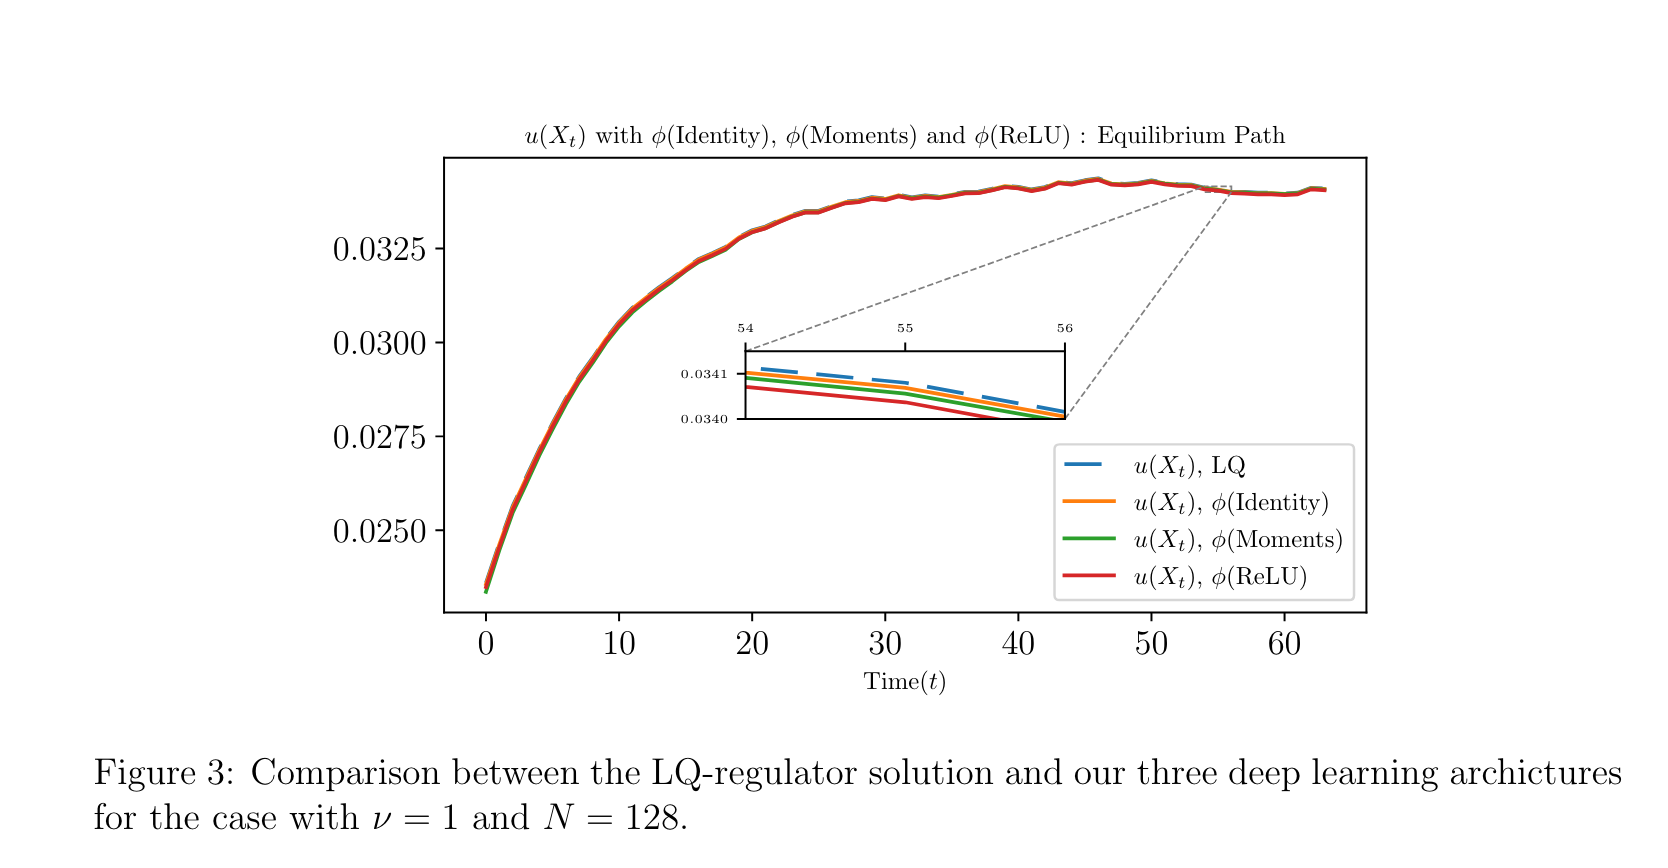
\includegraphics[width = 0.8\textwidth]{3.png}
\end{figure}
\end{frame}

\begin{frame}{Deep Learning Implementation}
\begin{figure}[h!]
\centering
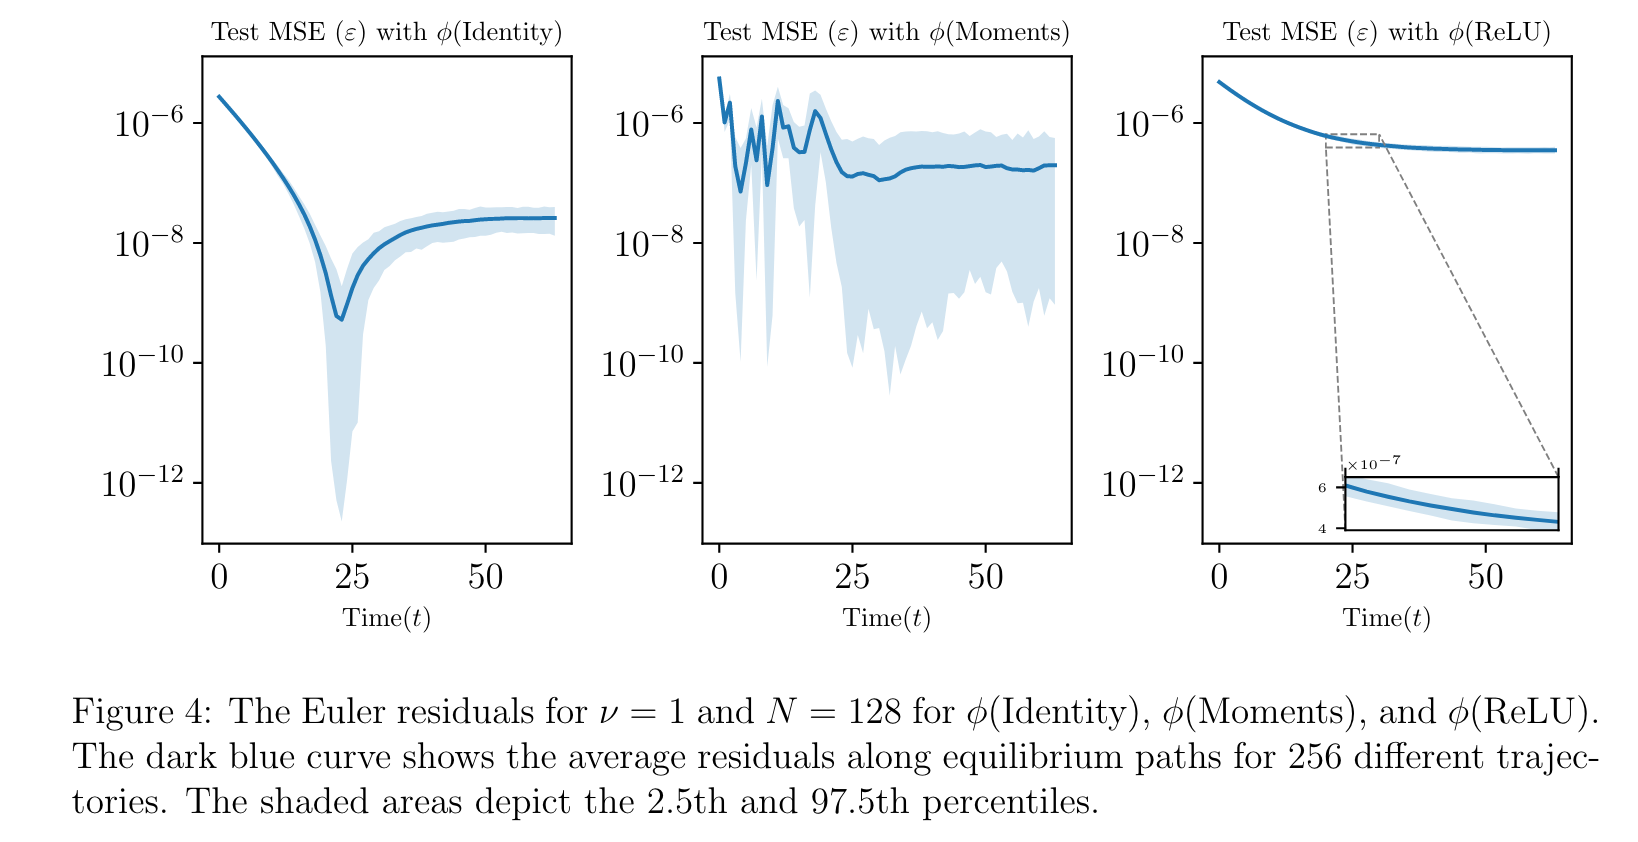
\includegraphics[width = 0.8\textwidth]{4.png}
\end{figure}
\end{frame}

\begin{frame}{Deep Learning Implementation}
\begin{figure}[h!]
\centering
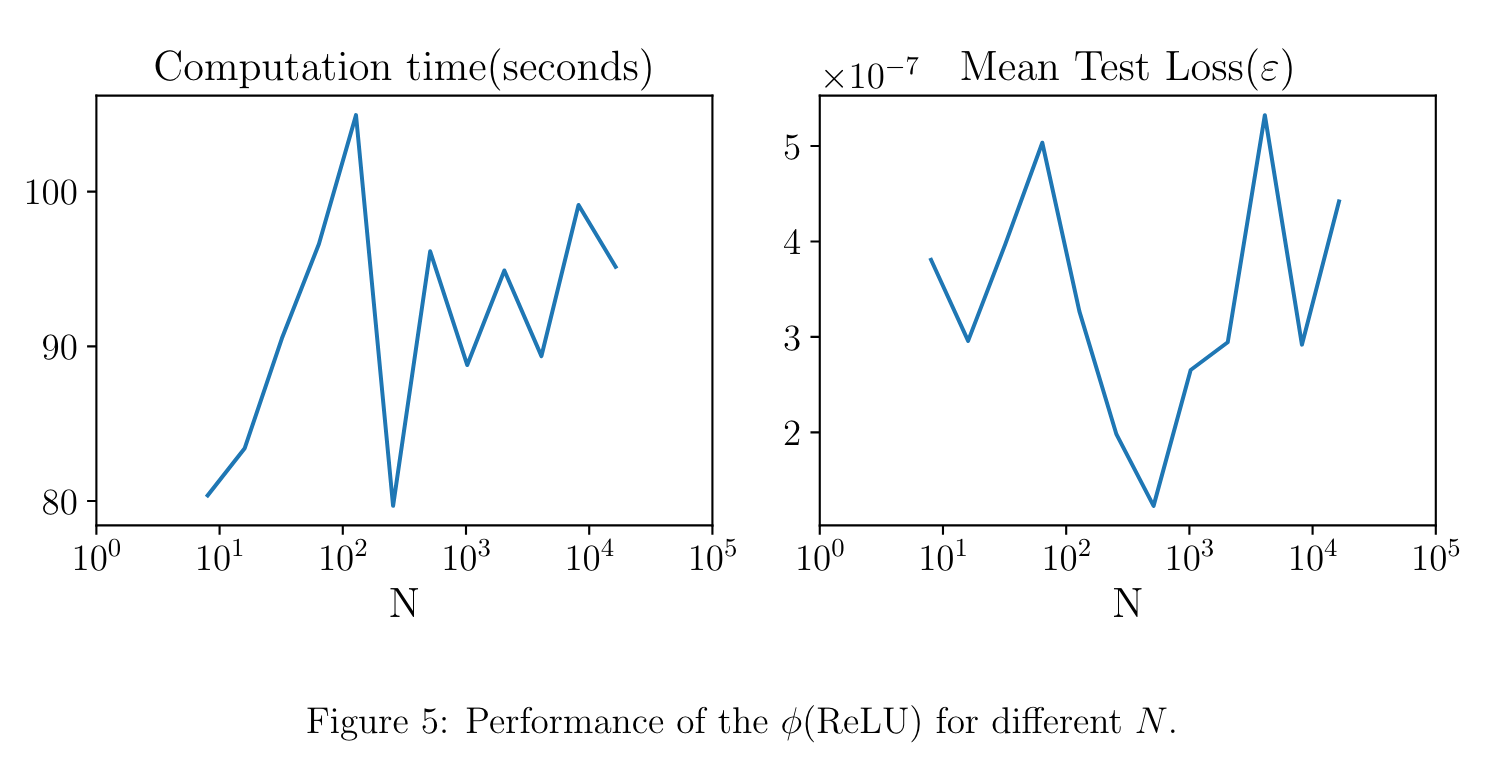
\includegraphics[width = 0.8\textwidth]{5.png}
\end{figure}
\end{frame}

\begin{frame}{Deep Learning Implementation}
\begin{figure}[h!]
\centering
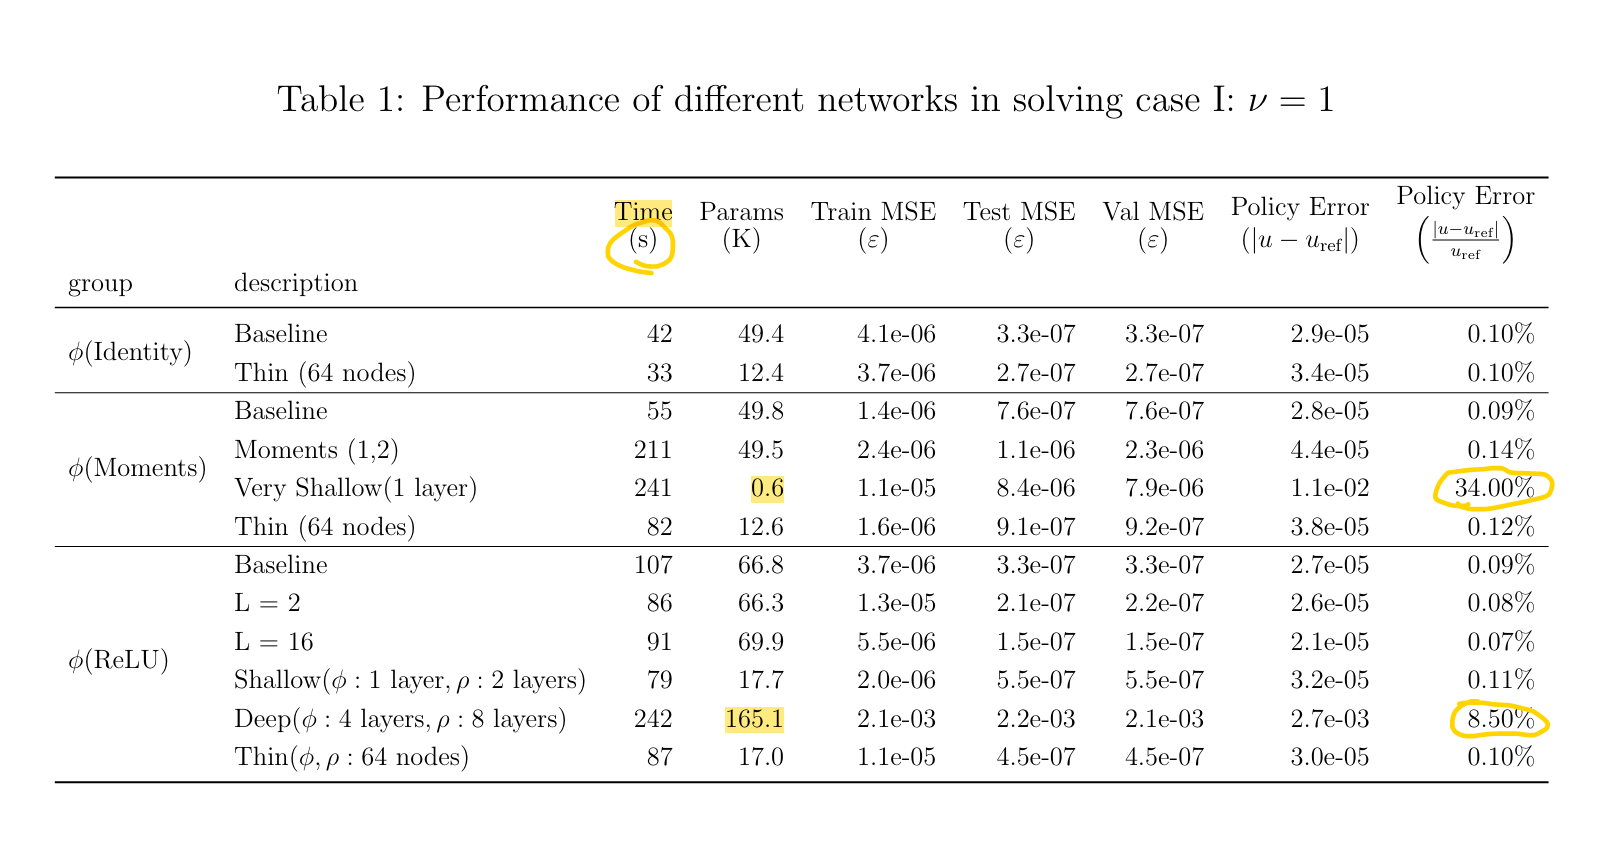
\includegraphics[width = \textwidth]{6.png}
\end{figure}
\end{frame}

\begin{frame}{Deep Learning Implementation}
Case II: 
\end{frame}

\section{Extensions}
\begin{frame}{Extensions}
The tools are useful for solving any high-dimensional functional equations with some degree of symmetry, especially when these equations contain high-dimensional expectations.
    \begin{itemize}
        \item Decreasing returns to scale\\
        \vspace{0.2cm}
        \item Multiple productivity types\\
        \vspace{0.2cm}
        \item Complex idiosyncratic states\\
        \vspace{0.2cm}
        \item Global solutions with transitions and aggregate shocks

    \end{itemize}
\end{frame}

\section{Discussion}
\begin{frame}{Discussion}
    \begin{itemize}
        \item Solve high-dimensional dynamic programming problems in minutes.
        \vspace{0.2cm}
        \item Double-descent
        \vspace{0.2cm}
        \item Model selection since results are sensitive to different network architectures. 
    \end{itemize}
\end{frame}
\end{document}